% !TeX root = main.tex
\section{Installing and Testing OpenCV}

Main docs: \url{https://docs.opencv.org/4.x/}
\\ \noindent
Python docs: \url{https://docs.opencv.org/4.x/d6/d00/tutorial_py_root.html}

% Installation and setup
\subsection{OpenCV Setup}

The procedure to setup OpenCV using Anaconda on windows is listed below

\begin{enumerate}
    \item Download and install Anaconda from \href{https://www.anaconda.com/products/individual}{here}.

    \item Setup the anaconda environment for the shell using \texttt{conda init}

    \item Setup the environment
    
        Create the environment
        \begin{verbatim}
            conda create -yn "cv-cs7-505"
            conda activate cv-cs7-505
        \end{verbatim}

        Install Python 3.9 into it
        \begin{verbatim}
            conda install python=3.9
        \end{verbatim}

        Install the essential packages (before OpenCV)
        \begin{verbatim}
            conda install numpy jupyterlab
        \end{verbatim}

    \item Install OpenCV using \texttt{pip}
    
        Install using pip
        \begin{verbatim}
            pip install opencv-python opencv-contrib-python
        \end{verbatim}

\end{enumerate}

\subsection{Testing Installation of OpenCV}

\subsubsection*{Checking Version}

Check version using the script below

\lstinputlisting[language=python]{../python/check_cv2_version.py}

The output of the above script is
\begin{verbatim}
    OpenCV version: 4.5.5
    Numpy version: 1.21.2
\end{verbatim}

\subsubsection*{Reading and changing color channels}

Consider the images in figure \ref{fig:q1-test-imgs}. The code to get this output is given below

\begin{figure}
    \centering
    \begin{subfigure}[b]{0.4\textwidth}
        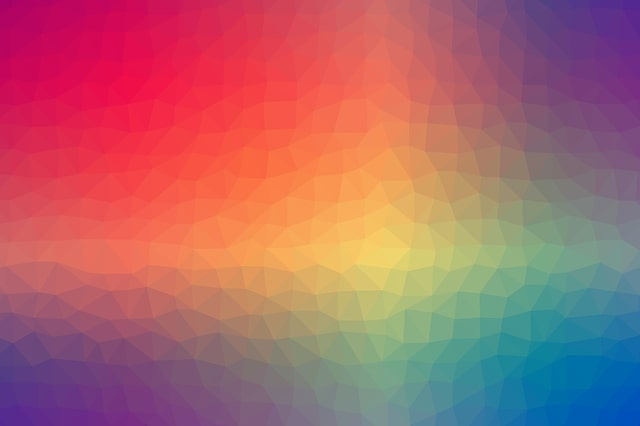
\includegraphics[width=\textwidth]{test.jpg}
        \caption{Input}
        \label{fig:sfig-test-in}
    \end{subfigure}
    \begin{subfigure}[b]{0.4\textwidth}
        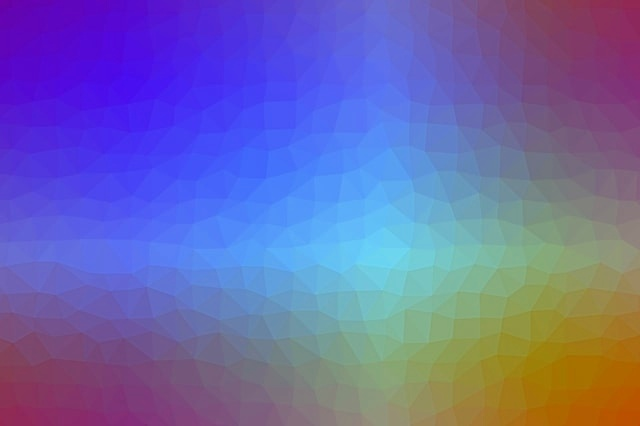
\includegraphics[width=\textwidth]{output.jpg}
        \caption{Output}
        \label{fig:sfig-test-out}
    \end{subfigure}
    \caption{Test images}
    \label{fig:q1-test-imgs}
    \small
        The red and blue channels are flipped (their layer intensities are swapped). Check code listing \ref{lst:q1-transform-img}
\end{figure}

\lstinputlisting[language=python, label=lst:q1-transform-img, caption=Transform images]{../python/transform_img.py}
